\documentclass{standalone}
\usepackage{tikz}
\usetikzlibrary{patterns, positioning}


\begin{document}
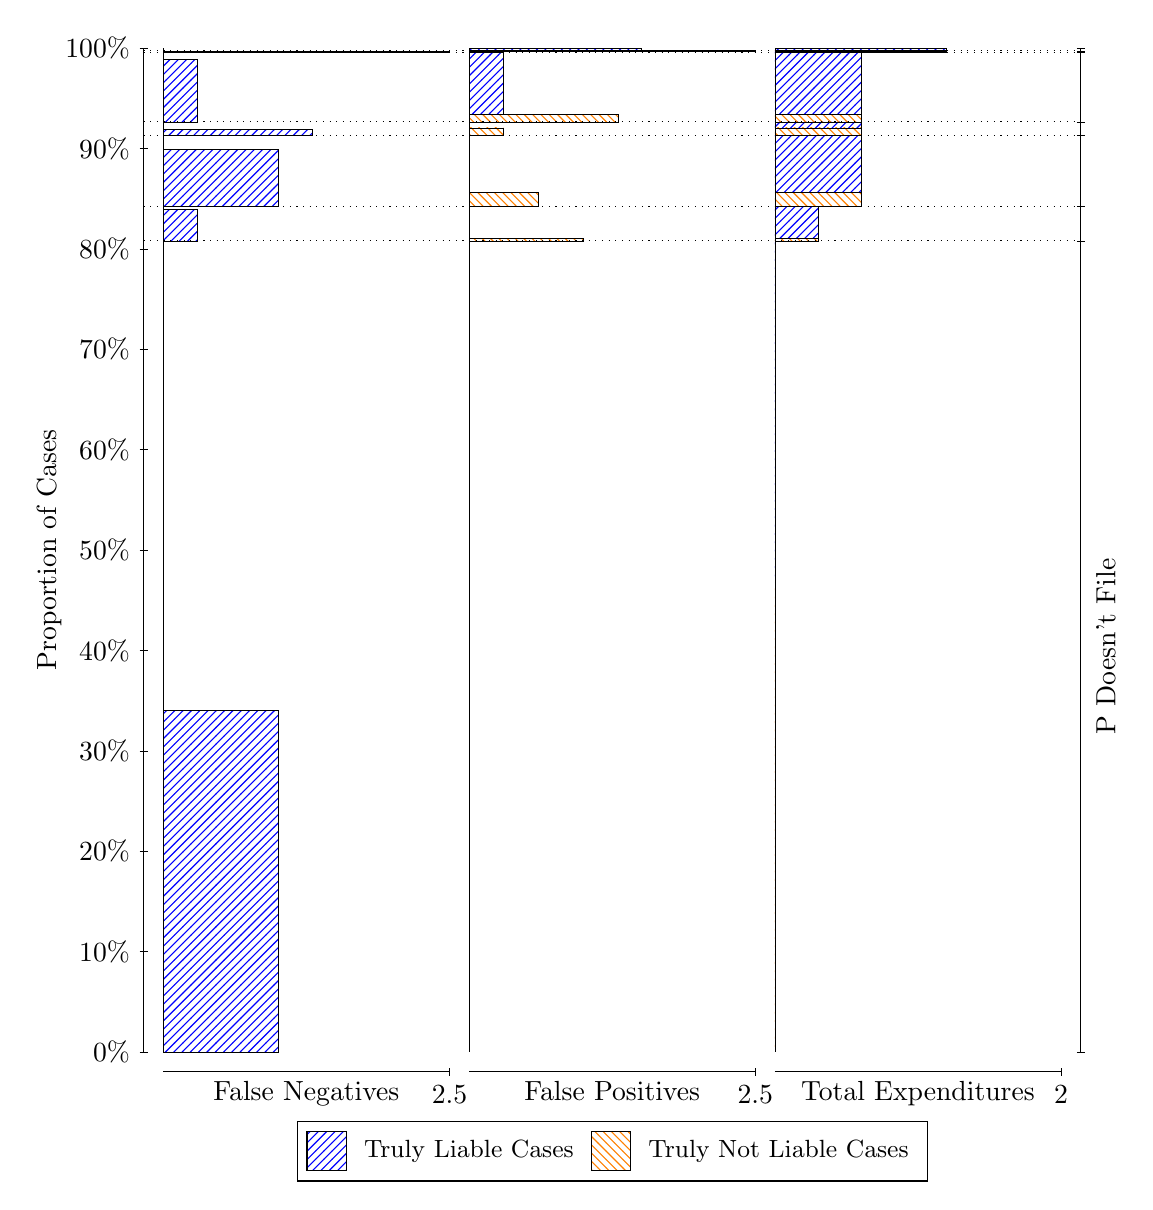
\begin{tikzpicture}
\draw[black, very thin] (1.5,1.75) -- (1.5,14.5);
\node[rotate=90, text=black, anchor=center] at (0.3, 8.125) {Proportion of Cases};
\draw[black, very thin] (1.45,1.75) -- (1.55,1.75);
\node[text=black, anchor=east] at (1.45, 1.75) {0\%};
\draw[black, very thin] (1.45,3.025) -- (1.55,3.025);
\node[text=black, anchor=east] at (1.45, 3.025) {10\%};
\draw[black, very thin] (1.45,4.3) -- (1.55,4.3);
\node[text=black, anchor=east] at (1.45, 4.3) {20\%};
\draw[black, very thin] (1.45,5.575) -- (1.55,5.575);
\node[text=black, anchor=east] at (1.45, 5.575) {30\%};
\draw[black, very thin] (1.45,6.85) -- (1.55,6.85);
\node[text=black, anchor=east] at (1.45, 6.85) {40\%};
\draw[black, very thin] (1.45,8.125) -- (1.55,8.125);
\node[text=black, anchor=east] at (1.45, 8.125) {50\%};
\draw[black, very thin] (1.45,9.4) -- (1.55,9.4);
\node[text=black, anchor=east] at (1.45, 9.4) {60\%};
\draw[black, very thin] (1.45,10.675) -- (1.55,10.675);
\node[text=black, anchor=east] at (1.45, 10.675) {70\%};
\draw[black, very thin] (1.45,11.95) -- (1.55,11.95);
\node[text=black, anchor=east] at (1.45, 11.95) {80\%};
\draw[black, very thin] (1.45,13.225) -- (1.55,13.225);
\node[text=black, anchor=east] at (1.45, 13.225) {90\%};
\draw[black, very thin] (1.45,14.5) -- (1.55,14.5);
\node[text=black, anchor=east] at (1.45, 14.5) {100\%};

\draw[black, very thin] (13.4,1.75) -- (13.4,14.5);
\draw[black, very thin] (13.35,1.75) -- (13.45,1.75);
\node[anchor=west] at (13.35, 1.75) {};
\draw[black, very thin] (13.35,12.052) -- (13.45,12.052);
\node[anchor=west] at (13.35, 12.052) {};
\draw[black, very thin] (13.35,12.489) -- (13.45,12.489);
\node[anchor=west] at (13.35, 12.489) {};
\draw[black, very thin] (13.35,13.392) -- (13.45,13.392);
\node[anchor=west] at (13.35, 13.392) {};
\draw[black, very thin] (13.35,13.563) -- (13.45,13.563);
\node[anchor=west] at (13.35, 13.563) {};
\draw[black, very thin] (13.35,14.445) -- (13.45,14.445);
\node[anchor=west] at (13.35, 14.445) {};
\draw[black, very thin] (13.35,14.464) -- (13.45,14.464);
\node[anchor=west] at (13.35, 14.464) {};
\draw[black, very thin] (13.35,14.5) -- (13.45,14.5);
\node[anchor=west] at (13.35, 14.5) {};

\draw[black, very thin, pattern color=blue, pattern=north east lines] (1.75,1.75) rectangle (3.2033,6.093);
\draw[black, very thin, pattern color=orange, pattern=north west lines] (1.75,6.093) rectangle (1.75,12.052);
\draw[black, very thin, pattern color=blue, pattern=north east lines] (1.75,12.052) rectangle (2.186,12.455);
\draw[black, very thin, pattern color=orange, pattern=north west lines] (1.75,12.455) rectangle (1.75,12.489);
\draw[black, very thin, pattern color=blue, pattern=north east lines] (1.75,12.489) rectangle (3.2033,13.213);
\draw[black, very thin, pattern color=orange, pattern=north west lines] (1.75,13.213) rectangle (1.75,13.392);
\draw[black, very thin, pattern color=blue, pattern=north east lines] (1.75,13.392) rectangle (3.6393,13.469);
\draw[black, very thin, pattern color=orange, pattern=north west lines] (1.75,13.469) rectangle (1.75,13.563);
\draw[black, very thin, pattern color=blue, pattern=north east lines] (1.75,13.563) rectangle (2.186,14.355);
\draw[black, very thin, pattern color=orange, pattern=north west lines] (1.75,14.355) rectangle (1.75,14.445);
\draw[black, very thin, pattern color=blue, pattern=north east lines] (1.75,14.445) rectangle (5.3833,14.454);
\draw[black, very thin, pattern color=orange, pattern=north west lines] (1.75,14.454) rectangle (1.75,14.464);
\draw[black, very thin, pattern color=orange, pattern=north west lines] (1.75,14.464) rectangle (1.75,14.473);
\draw[black, very thin, pattern color=blue, pattern=north east lines] (1.75,14.473) rectangle (1.75,14.5);
\draw[black, very thin, pattern color=orange, pattern=north west lines] (5.6333,1.75) rectangle (5.6333,7.7091);
\draw[black, very thin, pattern color=blue, pattern=north east lines] (5.6333,7.7091) rectangle (5.6333,12.052);
\draw[black, very thin, pattern color=orange, pattern=north west lines] (5.6333,12.052) rectangle (7.0867,12.086);
\draw[black, very thin, pattern color=blue, pattern=north east lines] (5.6333,12.086) rectangle (5.6333,12.489);
\draw[black, very thin, pattern color=orange, pattern=north west lines] (5.6333,12.489) rectangle (6.5053,12.668);
\draw[black, very thin, pattern color=blue, pattern=north east lines] (5.6333,12.668) rectangle (5.6333,13.392);
\draw[black, very thin, pattern color=orange, pattern=north west lines] (5.6333,13.392) rectangle (6.0693,13.486);
\draw[black, very thin, pattern color=blue, pattern=north east lines] (5.6333,13.486) rectangle (5.6333,13.563);
\draw[black, very thin, pattern color=orange, pattern=north west lines] (5.6333,13.563) rectangle (7.5227,13.653);
\draw[black, very thin, pattern color=blue, pattern=north east lines] (5.6333,13.653) rectangle (6.0693,14.445);
\draw[black, very thin, pattern color=orange, pattern=north west lines] (5.6333,14.445) rectangle (5.6333,14.454);
\draw[black, very thin, pattern color=blue, pattern=north east lines] (5.6333,14.454) rectangle (5.6333,14.464);
\draw[black, very thin, pattern color=orange, pattern=north west lines] (5.6333,14.464) rectangle (9.2667,14.473);
\draw[black, very thin, pattern color=blue, pattern=north east lines] (5.6333,14.473) rectangle (7.8133,14.5);
\draw[black, very thin, pattern color=orange, pattern=north west lines] (9.5167,1.75) rectangle (9.5167,7.7091);
\draw[black, very thin, pattern color=blue, pattern=north east lines] (9.5167,7.7091) rectangle (9.5167,12.052);
\draw[black, very thin, pattern color=orange, pattern=north west lines] (9.5167,12.052) rectangle (10.062,12.086);
\draw[black, very thin, pattern color=blue, pattern=north east lines] (9.5167,12.086) rectangle (10.062,12.489);
\draw[black, very thin, pattern color=orange, pattern=north west lines] (9.5167,12.489) rectangle (10.607,12.668);
\draw[black, very thin, pattern color=blue, pattern=north east lines] (9.5167,12.668) rectangle (10.607,13.392);
\draw[black, very thin, pattern color=orange, pattern=north west lines] (9.5167,13.392) rectangle (10.607,13.486);
\draw[black, very thin, pattern color=blue, pattern=north east lines] (9.5167,13.486) rectangle (10.607,13.563);
\draw[black, very thin, pattern color=orange, pattern=north west lines] (9.5167,13.563) rectangle (10.607,13.653);
\draw[black, very thin, pattern color=blue, pattern=north east lines] (9.5167,13.653) rectangle (10.607,14.445);
\draw[black, very thin, pattern color=orange, pattern=north west lines] (9.5167,14.445) rectangle (11.697,14.454);
\draw[black, very thin, pattern color=blue, pattern=north east lines] (9.5167,14.454) rectangle (11.697,14.464);
\draw[black, very thin, pattern color=orange, pattern=north west lines] (9.5167,14.464) rectangle (11.697,14.473);
\draw[black, very thin, pattern color=blue, pattern=north east lines] (9.5167,14.473) rectangle (11.697,14.5);
\draw[black, dotted] (1.5,12.052) -- (13.4,12.052);
\draw[black, dotted] (1.5,12.489) -- (13.4,12.489);
\draw[black, dotted] (1.5,13.392) -- (13.4,13.392);
\draw[black, dotted] (1.5,13.563) -- (13.4,13.563);
\draw[black, dotted] (1.5,14.445) -- (13.4,14.445);
\draw[black, dotted] (1.5,14.464) -- (13.4,14.464);
\draw[black, very thin] (1.75,1.5) -- (5.3833,1.5);
\node[text=black, anchor=north] at (3.5667, 1.5) {False Negatives};
\draw[black, very thin] (5.3833,1.45) -- (5.3833,1.55);
\node[text=black, anchor=north] at (5.3833, 1.45) {2.5};

\draw[black, very thin] (5.6333,1.5) -- (9.2667,1.5);
\node[text=black, anchor=north] at (7.45, 1.5) {False Positives};
\draw[black, very thin] (9.2667,1.45) -- (9.2667,1.55);
\node[text=black, anchor=north] at (9.2667, 1.45) {2.5};

\draw[black, very thin] (9.5167,1.5) -- (13.15,1.5);
\node[text=black, anchor=north] at (11.333, 1.5) {Total Expenditures};
\draw[black, very thin] (13.15,1.45) -- (13.15,1.55);
\node[text=black, anchor=north] at (13.15, 1.45) {2};

\node[text=black, centered, rotate=90] at (13.72, 6.901) {P Doesn't File};







\draw (7.449999999999999,1.5) node[draw=none] (baseCoordinate) {};
\begin{scope}[align=center]
        \matrix[scale=0.5, draw=black, below=0.5cm of baseCoordinate, nodes={draw}, column sep=0.1cm]{
            \node[rectangle, draw, minimum width=0.5cm, minimum height=0.5cm, pattern color=blue, pattern=north east lines] {}; &
            \node[draw=none, font=\small, text=black] (B) {Truly Liable Cases}; &
            \node[rectangle, draw, minimum width=0.5cm, minimum height=0.5cm, pattern color=orange, pattern=north west lines] {}; &
            \node[draw=none, font=\small, text=black] (B) {Truly Not Liable Cases}; \\
            };
\end{scope}

\end{tikzpicture}
\end{document}